\documentclass[9pt]{beamer}
\usepackage[utf8]{inputenc}
\usepackage[russian,english]{babel}
\usepackage{graphicx, epsfig}
\usepackage{amsmath,mathrsfs,amsfonts,amssymb}
\usepackage{subfig}
\usepackage{floatflt}
\usepackage{epic,ecltree}
\usepackage{mathtext}
\usepackage{fancybox}
\usepackage{fancyhdr}
\usepackage{multirow}
\usepackage{enumerate}
\usepackage{epstopdf}
\usepackage{multicol}
\usepackage{algorithm}
\usepackage[noend]{algorithmic}
\def\algorithmicrequire{\textbf{Input:}}
\def\algorithmicensure{\textbf{Output:}}
\usetheme{Singapore}%{Singapore}%{Warsaw}%{Warsaw}%{Darmstadt}
\usecolortheme{default}
\setbeamertemplate{footline}[page number]{}
\newcommand{\bx}{\mathbf{x}}
\newcommand{\by}{\mathbf{y}}
\newcommand{\bz}{\mathbf{z}}
\newcommand{\bw}{\mathbf{w}}
\newcommand{\ba}{\mathbf{a}}
\newcommand{\bb}{\mathbf{b}}
\newcommand{\bY}{\mathbf{Y}}
\newcommand{\bX}{\mathbf{X}}
\newcommand{\bu}{\mathbf{u}}
\newcommand{\bt}{\mathbf{t}}
\newcommand{\bp}{\mathbf{p}}
\newcommand{\bq}{\mathbf{q}}
\newcommand{\bc}{\mathbf{c}}
\newcommand{\bP}{\mathbf{P}}
\newcommand{\bT}{\mathbf{T}}
\newcommand{\bB}{\mathbf{B}}
\newcommand{\bQ}{\mathbf{Q}}
\newcommand{\bC}{\mathbf{C}}
\newcommand{\bE}{\mathbf{E}}
\newcommand{\bF}{\mathbf{F}}
\newcommand{\bU}{\mathbf{U}}
\newcommand{\bW}{\mathbf{W}}
\newcommand{\bbR}{\mathbb{R}}
\newcommand{\cA}{\mathcal{A}}
\newcommand{\bchi}{\boldsymbol{\chi}}
\newcommand{\bnu}{\boldsymbol{\nu}}
\newcommand{\bmu}{\boldsymbol{\mu}}
\newcommand{\bOne}{\boldsymbol{1}}
\newcommand{\bZero}{\boldsymbol{0}}
\newcommand{\btheta}{\boldsymbol{\theta}}
\newcommand{\bTheta}{\boldsymbol{\Theta}}
\newcommand{\argmin}{\mathop{\arg \min}\limits}
\newcommand{\argmax}{\mathop{\arg \max}\limits}
\newcommand{\T}{\mathsf{T}}

\newcommand\undermat[2]{%
	\makebox[0pt][l]{$\smash{\underbrace{\phantom{%
					\begin{matrix}#2\end{matrix}}}_{\text{$#1$}}}$}#2}

\newtheorem{statement}{Statement}

\titlegraphic{
\includegraphics[width=2cm]{figs/mipt_logo}~%
	
\includegraphics[width=2cm]{figs/sk_logo}
}

% отображать название слайда слева
\setbeamertemplate{frametitle}[default][left]

\usepackage{tikz-cd}
%\definecolor{beamer@blendedblue}{RGB}{15,120,80}
%----------------------------------------------------------------------------------------------------------
\title[\hbox to 56mm{  \hfill\insertframenumber\,/\,\inserttotalframenumber}]
{\\ \vspace{1.5cm} Dimensionality Reduction for Signal Analysis}
\author[Roman Isachenko]{\\ 
	\vspace{.4cm}
	Roman Isachenko}
\institute[SkolTech]{Skoltech advisor: Maxim Fedorov \\ 
	\vspace{0.1cm}
	 MIPT advisor: Vadim Strijov
}
\date{June 18, 2018.}
%--------------------------------------------------------------------------------
\begin{document}
%--------------------------------------------------------------------------------
\begin{frame}
%\thispagestyle{empty}
\titlepage
\end{frame}
%--------------------------------------------------------------------------------
\begin{frame}{Signal decoding problem}
	\begin{block}{Goal}
		Investigate dependencies in both input and target spaces and build a stable model for signal decoding in the case of multicorrelated object description.
	\end{block}
	\begin{block}{Challenge}
		\begin{itemize}
			\item Measurements of spatial-temporal data are interacted since sensors are close to each other.
			\item Target variable is a vector whose elements are dependent.
		\end{itemize}
	\end{block}
	\begin{block}{Solution}
		Propose dimensionality reduction and feature selection algorithms which take into account dependencies in both input and target spaces. 
	\end{block}
\end{frame}
%--------------------------------------------------------------------------------
\begin{frame}{Related works}
	\begin{itemize}
		\item Katrutsa A., Strijov V. Comprehensive study of feature selection methods to solve multicollinearity problem according to evaluation criteria // \textit{Expert Systems with Applications} 76, 2017.
		\vfill
		\item Li J. et al. Feature selection: A data perspective //\textit{ACM Computing Surveys (CSUR)} 50(6), 2017.
		\vfill
		\item Eliseyev A. et al. Iterative N-way partial least squares for a binary self-paced brain–computer interface in freely moving animals //\textit{Journal of neural engineering} 4(8), 2011.
		\vfill
		\item Rodriguez-Lujan I. et al. Quadratic programming feature selection // \textit{Journal of Machine Learning Research} 11(Apr), 2010.
		\vfill
		\item Motrenko A., Strijov V. Multi-way Feature Selection for ECoG-based Brain-Computer Interface // \textit{Expert Systems with Applications} Submitted to the journal.
	\end{itemize}
\end{frame}
%--------------------------------------------------------------------------------
\begin{frame}{Multivariate regression}
	\begin{block}{Given}
	Dataset $\left( \bX, \bY \right)$, design matrix~$\bX \in \bbR^{m \times n}$, target matrix~$\bY \in \bbR^{m \times r}$,
	\[
	\bX = [\bchi_1, \dots, \bchi_n]; \quad \bY =  [\bnu_1, \dots, \bnu_r].
	\]
	\vspace{-0.7cm}
	\end{block}

\begin{block}{Model}
	Forecast a dependent variable $\by \in \bbR^r$ from an independent input object $\bx \in \bbR^n$
	\[
	\by = \bTheta \bx+ \boldsymbol{\varepsilon}, \quad \bTheta \in \bbR^{r \times n}.
	\]
	\vspace{-0.7cm}
\end{block}
	\begin{block}{Loss function}
	\[
	\mathcal{L}(\bTheta | \bX, \bY) = {\left\| \underset{m \times r}{\mathbf{Y}}  - \underset{m \times n}{\bX} \cdot \underset{r \times n}{\bTheta}^{\T} \right\| }_2^2 \rightarrow\min_{\bTheta}.
	\label{eq:error_function}
	\]
	\[
	\bTheta^{\T} = (\bX^{\T} \bX)^{-1} \bX^{\T} \bY.
	\]
	\end{block}
	The linear dependent columns of the matrix $\bX$ leads to an instable solution. \\
	To avoid the strong linear dependence, dimensionality reduction and feature selection techniques are used.
\end{frame}
%--------------------------------------------------------------------------------
\begin{frame}{Dimensionality reduction}
\begin{block}{Goal}
	\begin{itemize}
		\item project the matrices $\bX$ and $\bY$ into joint latent space;
		\item maximize covariance between the projections;
		\item save variance of the initial matrices.
	\end{itemize}
\end{block}


\begin{block}{Partial Least Squares (PLS) regression}
	\vspace{-0.5cm}
	\begin{align*}
	\underset{m \times n}{\vphantom{\bQ}\bX} 
	&= \underset{m \times l}{\vphantom{\bQ}\bT} \cdot \underset{l \times n}{\vphantom{\bQ}\bP^{\T}} + \underset{m \times n}{\vphantom{\bQ}\bF} 
	= \sum_{k=1}^l \underset{m \times 1}{\vphantom{\bp_k^{\T}}\bt_k} \cdot \underset{1 \times n}{\bp_k^{\T}} + \underset{m \times n}{\vphantom{\bp_k^{\T}}\bF},\\
	\underset{m \times r}{\vphantom{\bQ}\bY} 
	&= \underset{m \times l}{\vphantom{\bQ}\bU} \cdot \underset{l \times r}{\bQ^{\T}} + \underset{m \times r}{\vphantom{\bQ}\bE}
	=  \sum_{k=1}^l  \underset{m \times 1}{\vphantom{\bq_k^{\T}}\bu_k} \cdot \underset{1 \times r}{\bq_k^{\T}} +  \underset{m \times r}{\vphantom{\bq_k^{\T}}\bE}.
	\end{align*}
	\begin{equation*}
	\bU \approx \bT \bB, \quad \bB = \text{diag}(\beta_k), \quad \beta_k = \bu_k^{\T}\bt_k / (\bt_k^{\T}\bt_k).
	\end{equation*}
\end{block}

\end{frame}
%--------------------------------------------------------------------------------
\begin{frame}{PLS pseudocode}

\begin{figure}
\begin{flushleft}
	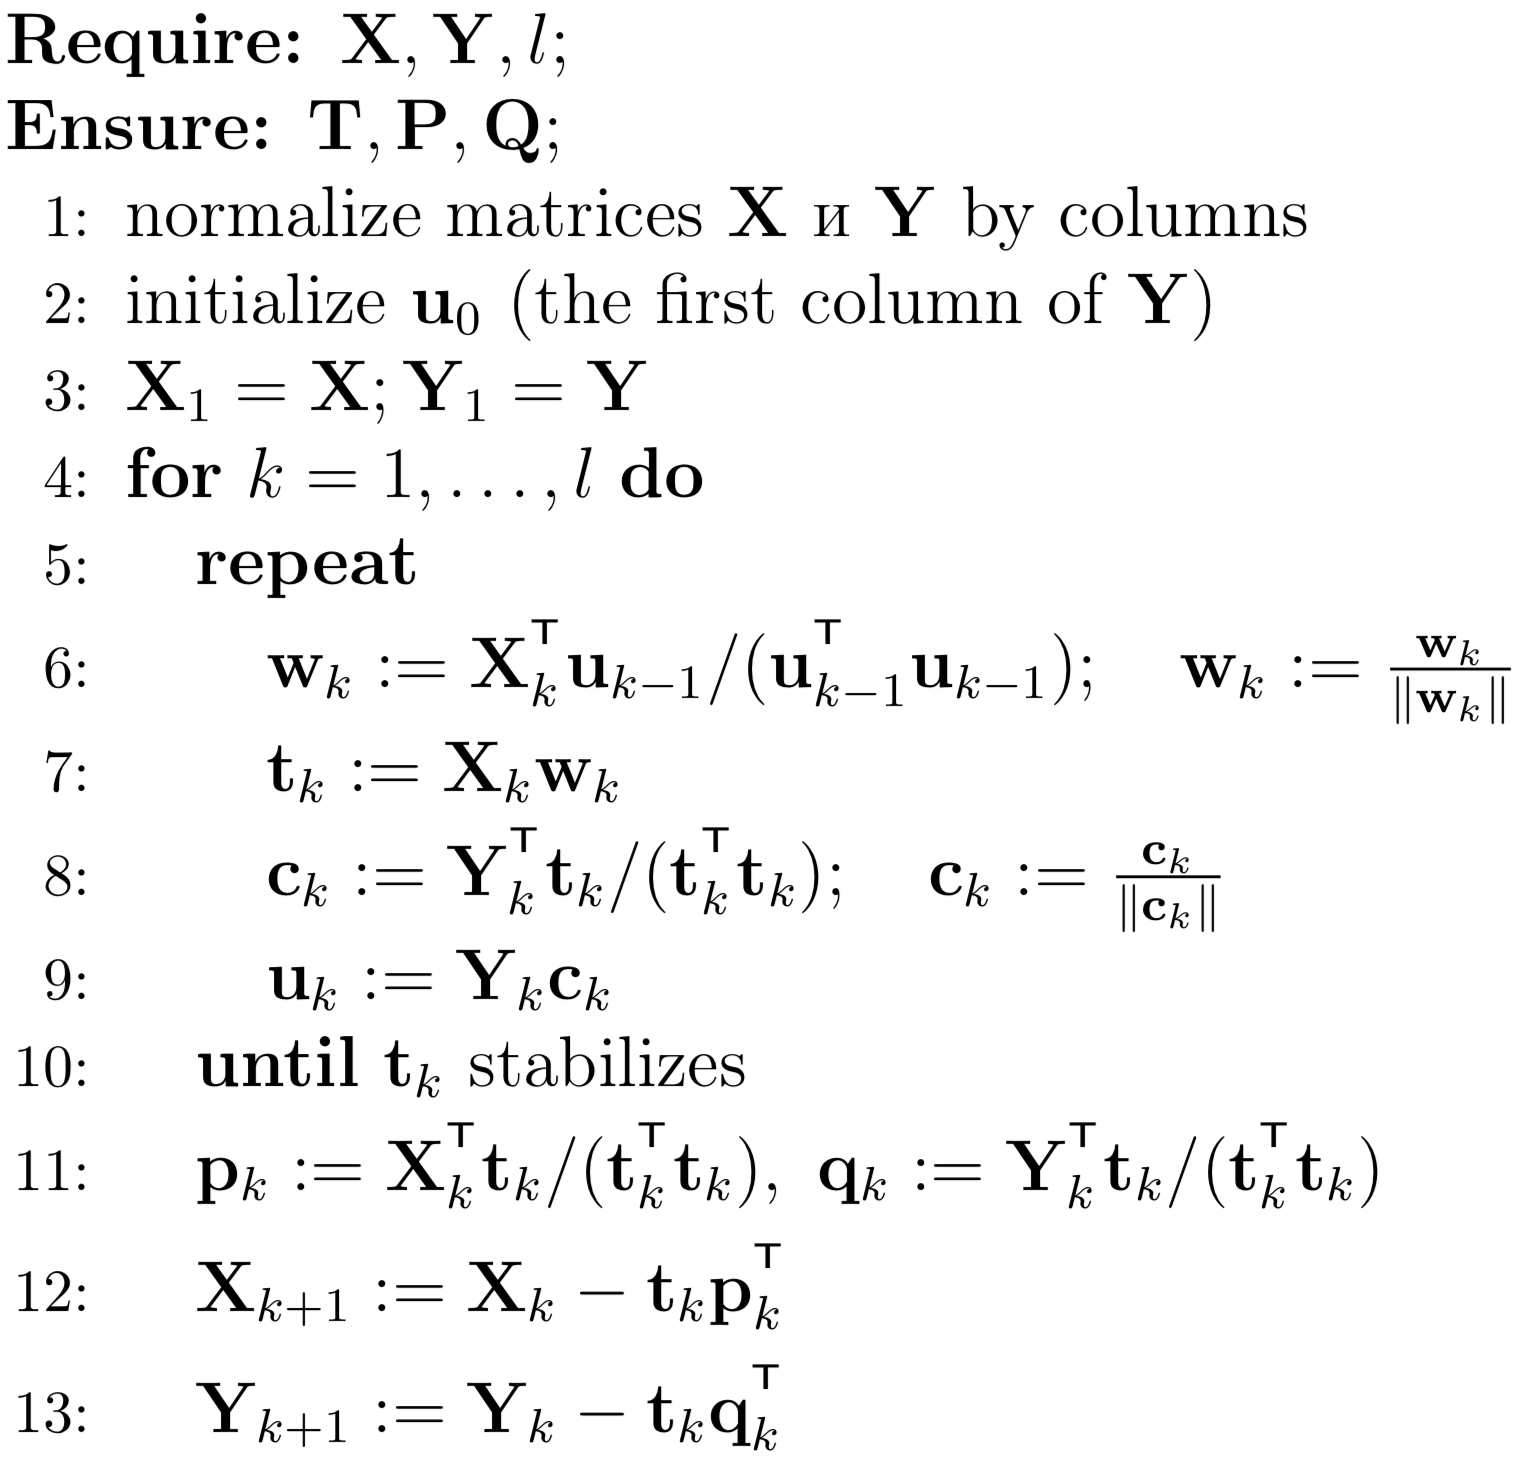
\includegraphics[width=0.6\linewidth]{figs/pls_pseudocode}
\end{flushleft}
\end{figure}
\end{frame}
%--------------------------------------------------------------------------------
\begin{frame}{PLS regression}

\begin{statement}[Isachenko, 2017]
The best description of the matrices $\bX$ and $\bY$ taking into account their interrelation is achieved by maximization of the covariance between the vectors $\bt_k$ and $\bu_k$.
\end{statement}
\begin{statement}[Isachenko, 2017]
	The vector $\bw_k$ and $\bc_k$ are eigenvectors of the matrices $\bX_k^{\T} \bY_k \bY_k^{\T} \bX_k$ and $\bY_k^{\T} \bX_k \bX_k^{\T} \bY_k$, corresponding to the maximum eigenvalues.
\end{statement}
\begin{statement}[Isachenko, 2017]
	The update rule for the vectors in steps (6)--(9) corresponds to the maximization of the covariance between the vectors $\bt_k$ and $\bu_k$.
\end{statement}

\begin{block}{PLS regression model}

\[
\bY = \bU \bQ^{\T} + \bE \approx \bT \bB \bQ^{\T}+ \bE = \bX \bW^* \bB \bQ^{\T} + \bE = \bX \bTheta + \bE.
\]
\[
\bTheta = \bW (\bP^{\T} \bW)^{-1} \bB \bQ^{\T}, \quad \bT = \bX \bW^*, \quad \text{where } \bW^* = \bW (\bP^{\T} \bW)^{-1}.
\]
\end{block}
\end{frame}
%--------------------------------------------------------------------------------
\begin{frame}{PLS example for two-dimensional case}
\begin{figure}[h]
\centering
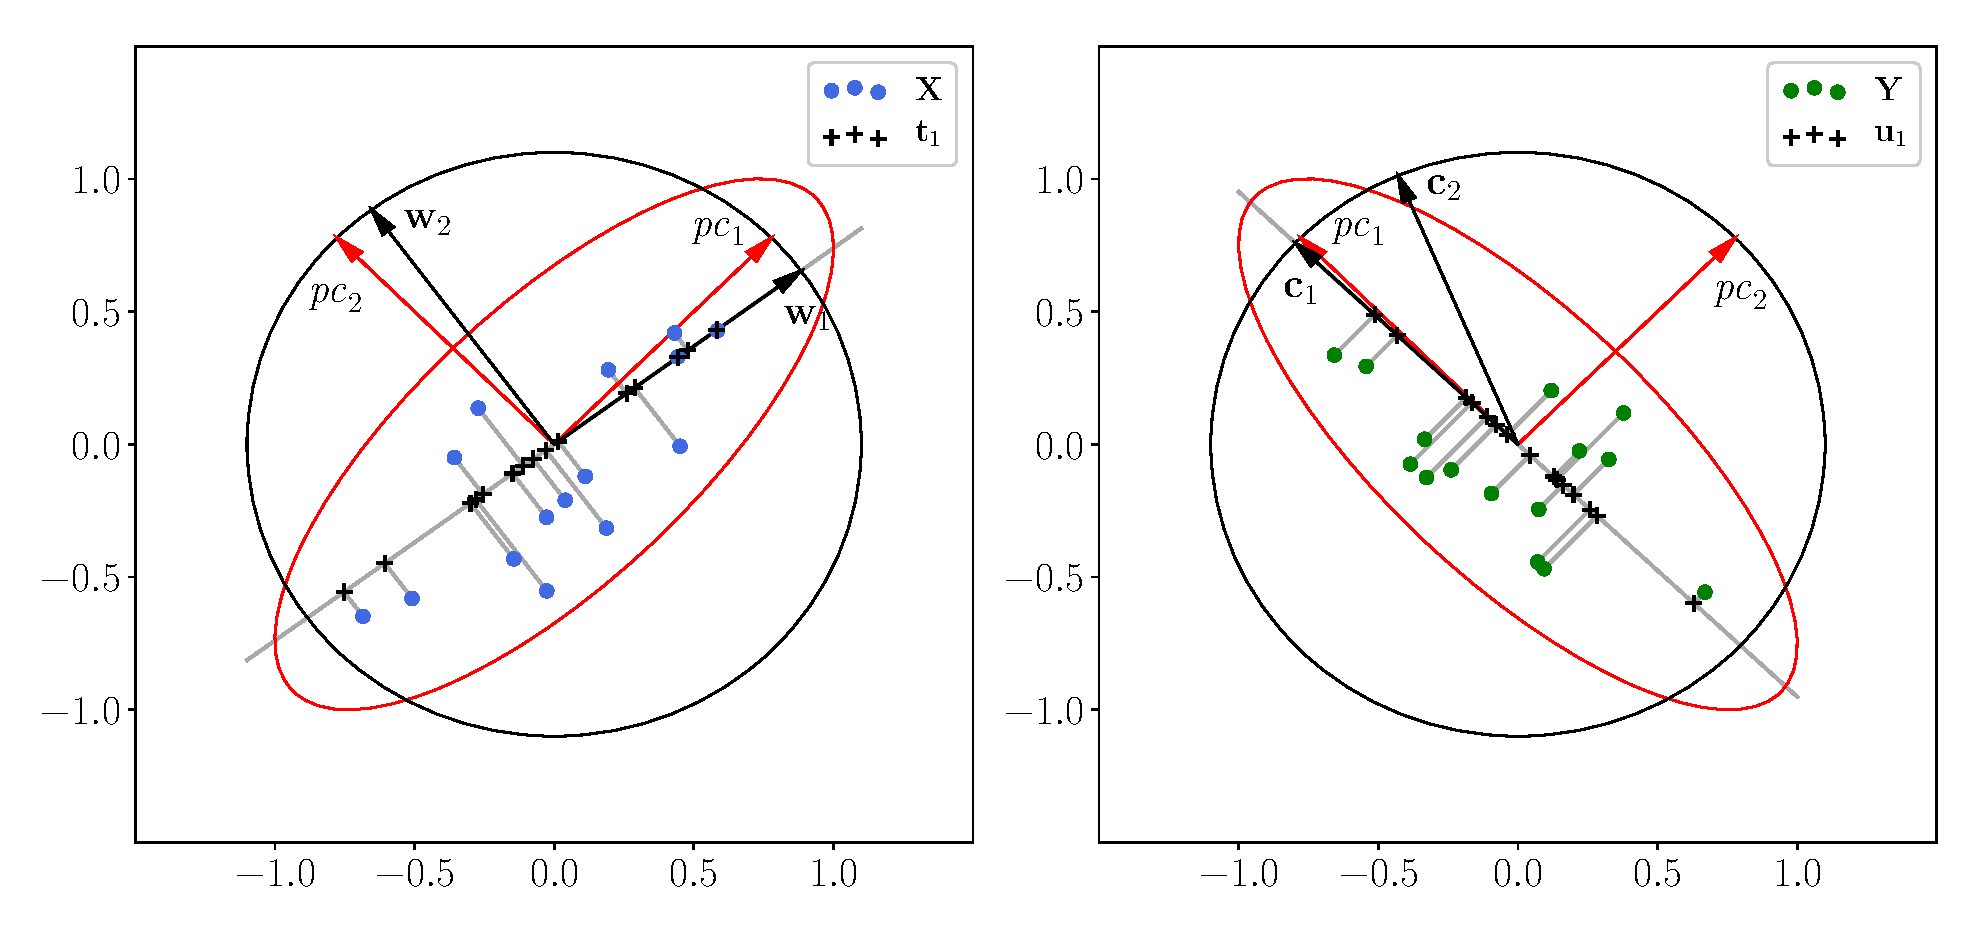
\includegraphics[width=\linewidth]{figs/PLSFigure.eps}
\end{figure}
\end{frame}
%--------------------------------------------------------------------------------
\begin{frame}{Feature selection problem}
\begin{block}{Goal}
Find a boolean vector~$\ba = \{0, 1\}^n$ of indicators for selected features. 
\end{block}
\begin{block}{Feature selection error function}
	\vspace{-0.2cm}
\[
\ba = \argmin_{\ba' \in \{0, 1\}^n} S(\ba' | \bX, \bY).
\]
\vspace{-0.5cm}
\end{block}
\begin{block}{Relaxed problem}
	From discrete domain $\{0, 1\}^n$ to continuous relaxation $[0, 1]^n$:
	\[
	\bz = \argmin_{\bz' \in [0, 1]^n} S(\bz' | \bX, \bY), \quad 
	a_j = [z_j > \tau].
\]
\end{block}
Once the solution~$\ba$ is known:
\[
\mathcal{L}(\bTheta_{\ba} | \bX_{\ba}, \bY) = {\left\| \mathbf{Y} - \bX_{\ba}\bTheta^{\T}_{\ba} \right\| }_2^2 \rightarrow\min_{\bTheta_{\ba}},
\]
where the subscript~$\ba$ indicates the submatrix with the columns for which~$a_j = 1$.
\end{frame}
%--------------------------------------------------------------------------------
\begin{frame}{Quadratic Programming Feature Selection}
	\[
	\| \bnu - \bX \btheta\|_2^2 \rightarrow\min_{\btheta \in \bbR^{n}}.
	\]
	\vspace{-0.3cm}
	\begin{block}{Quadratic programming problem}
	\vspace{-0.3cm}
	\[
	S(\bz | \bX, \bnu)	= (1 - \alpha) \cdot \underbrace{\bz^{\T} \bQ \bz}_{\text{Sim}(\bX)} - \alpha \cdot \underbrace{\vphantom{()} \mathbf{b}^{\T} \bz}_{\text{Rel}(\bX, \bnu)} \rightarrow \min_{\substack{\bz \geq \bZero_n \\ \bOne_n^{\T} \bz=1}}.
	\]
	\end{block}
		\begin{itemize}
			\item $\bz \in [0, 1]^n$ -- feature importances;
			\item $\bQ \in \bbR^{n \times n}$ -- pairwise feature similarities;
			\item $\mathbf{b} \in \bbR^n$ -- feature relevances to the target vector.
		\end{itemize}
		\[
		\bQ = \left[\left|\text{corr}(\bchi_i, \bchi_j)\right|\right]_{i,j=1}^n, \quad
		\bb = \left[\left|\text{corr}(\bchi_i, \bnu)\right|\right]_{i=1}^n.
		\]
\vspace{-0.2cm}
\begin{block}{Statement}
	In the case of semidefinite matrix $\bQ$ the QPFS problem is convex. Shift spectrum for semidefinite relaxation:
\end{block}
\begin{equation*}
\bQ \rightarrow \bQ - \lambda_{\min} \mathbf{I}.
\end{equation*}
\end{frame}
%--------------------------------------------------------------------------------
\begin{frame}{Multivariate QPFS}
\begin{block}{Relevance Aggregation (RelAgg)}
	\[
	\bb = \left[\left|\text{corr}(\bchi_i, \bnu)\right|\right]_{i=1}^n \rightarrow \bb = \left[\sum_{k=1}^r\left|\text{corr}(\bchi_i, \bnu_k)\right|\right]_{i=1}^n.
	\]
\end{block}
{\bf Drawback:} the approach does not use the dependencies in the columns of~$\bY$. 

\begin{block}{Symmetric Importances (SymImp)}
	Penalize correlated targets by $\text{Sim} (\bY)$
	\[
	\alpha_1 \cdot \underbrace{\bz_x^{\T} \bQ_x \bz_x}_{\text{Sim}(\bX)} - \alpha_2 \cdot \underbrace{\bz_x^{\T} \bB \bz_y}_{\text{Rel}(\bX, \bY)} + \alpha_3 \cdot \underbrace{\bz_y^{\T} \bQ_y \bz_y}_{\text{Sim}(\bY)} \rightarrow \min_{\substack{\bz_x \geq \bZero_n, \, \bOne_n^{\T}\bz_x=1 \\ \bz_y \geq \bZero_r, \, \bOne_r^{\T}\bz_y=1}}.
	\]
	\[
	\bQ_x = \left[ \left| \text{corr}(\bchi_i, \bchi_j) \right| \right]_{i,j=1}^n, \,
	\bQ_y = \left[ \left| \text{corr}(\bnu_i, \bnu_j) \right| \right]_{i,j=1}^r, \,
	\bB =  \left[ \left| \text{corr}(\bchi_i, \bnu_j) \right| \right]_{\substack{i=1, \dots, n \\ j=1, \dots, r}}.
	\]
	\[
	\alpha_1 + \alpha_2 + \alpha_3 = 1, \quad \alpha_i \geq 0.
	\] 
\end{block}
\end{frame}
%--------------------------------------------------------------------------------
\begin{frame}{Multivariate QPFS}
SymImp penalizes targets that are correlated and are explained by features to a lesser extent. 
\[
\alpha_1 \cdot \underbrace{\bz_x^{\T} \bQ_x \bz_x}_{\text{Sim}(\bX)} - \alpha_2 \cdot \underbrace{\vphantom{()} \bz_x^{\T}\mathbf{B} \bz_y}_{\text{Rel}(\bX, \bY)} \rightarrow \min_{\substack{\bz_x \geq \bZero_n \\ \bOne_n^{\T}\bz_x=1}}; \quad
\alpha_3 \cdot \underbrace{\bz_y^{\T} \bQ_y \bz_y}_{\text{Sim}(\bY)} + \alpha_2 \cdot \underbrace{\vphantom{()} \bz_x^{\T} \mathbf{B} \bz_y}_{\text{Rel}(\bX, \bY)} \rightarrow \min_{\substack{\bz_y \geq \bZero_r  \\ \bOne_r^{\T}\bz_y=1}}.
\]
\vspace{-0.2cm}
\begin{block}{Minimax approach (MinMax)}
\vspace{-0.5cm}
\[
\min_{\substack{\bz_x \geq \bZero_n \\ \bOne_n^{\T}\bz_x=1}} 	\max_{\substack{\bz_y \geq \bZero_r \\ \bOne_r^{\T}\bz_y=1}} \left(\text {or} \, \max_{\substack{\bz_y \geq \bZero_r \\ \bOne_r^{\T}\bz_y=1}} \min_{\substack{\bz_x \geq \bZero_n \\ \bOne_n^{\T}\bz_x=1}}\right) \left[\alpha_1 \cdot \underbrace{\bz_x^{\T} \bQ_x \bz_x}_{\text{Sim}(\bX)} - \alpha_2 \cdot \underbrace{\bz_x^{\T} \bB \bz_y}_{\text{Rel}(\bX, \bY)} - \alpha_3 \cdot \underbrace{\bz_y^{\T} \bQ_y \bz_y}_{\text{Sim}(\bY)}\right].
\]
\end{block}
\vspace{-0.4cm}
\begin{theorem}[Isachenko, 2018]
	For positive definite matrices $\bQ_x$ and $\bQ_y$ the maxmin and minmax problems have the same optimal value. 
\end{theorem}
\vspace{-0.2cm}
\begin{theorem}[Isachenko, 2018]
	Minimax problem is equivalent to the quadratic problem with $n + r + 1$ variables.
\end{theorem}
Shift spectrum to obtain the convex semidefinite relaxation.

\end{frame}
%--------------------------------------------------------------------------------
\begin{frame}{Multivariate QPFS}
\begin{block}{Maximum Relevances (MaxRel)}
\[
\min_{\substack{\bz_x \geq \bZero_n \\ \bOne_n^{\T}\bz_x=1}} 	\max_{\substack{\bz_y \geq \bZero_r \\ \bOne_r^{\T}\bz_y=1}} \left[ (1 - \alpha) \cdot \bz_x^{\T} \bQ_x \bz_x - \alpha \cdot \bz_x^{\T} \bB \bz_y \right].
\]
\end{block}
\begin{theorem}[Isachenko, 2018]
	For positive definite matrices $\bQ_x$ the max-min and min-max problems have the same optimal value and the final quadratic problem is convex. 
\end{theorem}
\begin{block}{Assymmetric importances (AsymImp)}
\begin{equation*}
	\alpha_1 \cdot \underbrace{\bz_x^{\T} \bQ_x \bz_x}_{\text{Sim}(\bX)} - \alpha_2 \cdot  \underbrace{\left(\bz_x^{\T} \bB \bz_y - \bb^{\T} \bz_y \right) }_{\text{Rel}(\bX, \bY)} + \alpha_3 \cdot \underbrace{\bz_y^{\T} \bQ_y \bz_y}_{\text{Sim}(\bY)} \rightarrow \min_{\substack{\bz_x \geq \bZero_n, \, \bOne_n^{\T}\bz_x=1 \\ \bz_y \geq \bZero_r, \, \bOne_r^{\T}\bz_y=1}}.
\end{equation*}
For $b_j = \max\limits_{i=1, \dots n} [\bB]_{i, j}$ coefficients of~$\bz_y$ in~$\text{Rel}(\bX, \bY)$ are non-negative.

\begin{statement}
	For the univariate case $r=1$ the proposed strategies SymImp, MinMax, MaxRel, AsymImp coincide with the original QPFS algorithm.
\end{statement}
\end{block}
\end{frame}
%--------------------------------------------------------------------------------
\begin{frame}{Summary of the proposed algorithms}
\begin{table}
	\centering
	\footnotesize{
		\begin{tabular}{c|c|c}
			\hline
			Algorithm & Problem & Error function $S(\bz | \bX, \bY)$ \\
			\hline && \\ 
			RelAgg & $\min \bigl[ \text{Sim}(\bX) - \text{Rel}(\bX, \bY) \bigr] $ & $\min\limits_{\bz_x} \bigl[ (1 - \alpha) \cdot \bz_x^{\T} \bQ_x \bz_x - \alpha \cdot \bz_x^{\T} \bB \bOne_r \bigr] $ \\ &&\\
			SymImp & $\begin{aligned} \min \, \bigl[ \text{Sim}(\bX) & - \text{Rel}(\bX, \bY) \\ & + \text{Sim}(\bY) \bigr] \end{aligned}$ & $ \min\limits_{\bz_x, \, \bz_y} \left[ \alpha_1 \cdot \bz_x^{\T} \bQ_x \bz_x - \alpha_2 \cdot \bz_x^{\T} \bB \bz_y + \alpha_3 \cdot \bz_y^{\T} \bQ_y \bz_y \right] $\\ &&\\ 
			MinMax & $\begin{aligned} &\min \, \bigl[ \text{Sim}(\bX) - \text{Rel}(\bX, \bY) \bigr]  \\ & \max \bigl[\text{Rel}(\bX, \bY) + \text{Sim}(\bY) \bigr] \end{aligned}$ & $	\min\limits_{\bz_x} 	\max\limits_{\bz_y} \bigl[\alpha_1 \cdot \bz_x^{\T} \bQ_x \bz_x - \alpha_2 \cdot \bz_x^{\T} \bB \bz_y - \alpha_3 \cdot \bz_y^{\T} \bQ_y \bz_y \bigr]$ \\ &&\\ 
			MaxRel & $\begin{aligned} &\min \, \bigl[ \text{Sim}(\bX) - \text{Rel}(\bX, \bY) \bigr]  \\ & \max \bigl[\text{Rel}(\bX, \bY) \bigr] \end{aligned}$& $\min\limits_{\bz_x} 	\max\limits_{\bz_y} \bigl[ (1 - \alpha) \cdot \bz_x^{\T} \bQ_x \bz_x - \alpha \cdot \bz_x^{\T} \bB \bz_y \bigr]$ \\ 		&&\\
			AsymImp & $\begin{aligned} & \min \, \bigl[ \text{Sim}(\bX) - \text{Rel}(\bX, \bY) \bigr]\\ &  \max \bigl[\text{Rel}(\bX, \bY) + \text{Sim}(\bY) \bigr] \end{aligned}$ & $\min\limits_{\bz_x, \bz_y} \bigl[ \alpha_1 \bz_x^{\T} \bQ_x \bz_x - \alpha_2 \left(\bz_x^{\T} \bB \bz_y - \bb^{\T} \bz_y \right) + \alpha_3  \bz_y^{\T} \bQ_y \bz_y \bigr]$\\  && \\
			\hline
	\end{tabular}}
\end{table}
\end{frame}
%--------------------------------------------------------------------------------
\begin{frame}{Quality criteria}

\begin{block}{Scaled RMSE}
	Prediction quality:
	\[
	\text{sRMSE}(\bY, \widehat{\bY}_{\ba}) = \sqrt{\frac{\text{MSE} (\bY, \widehat{\bY}_{\ba})}{\text{MSE} (\bY, \overline{\bY})}} =  \frac{\| \bY - \widehat{\bY}_{\ba} \|_2}{\| \bY - \overline{\bY} \|_2}, \quad \text{where} \quad \widehat{\bY}_{\ba} = \bX_{\ba} \bTheta_{\ba}^{\T}.
	\]
	$\overline{\bY}$ is a constant prediction.
\end{block}

\begin{block}{Multicorrelation}
	Mean value of miltiple correlation coefficient:
	\[
	R^2 = \frac{1}{r} \text{tr} \left( \bC^{\T} \mathbf{R}^{-1} \bC \right); \quad \bC = [ \text{corr}(\bchi_i, \bnu_j)]_{\substack{i=1, \dots, n \\ j=1, \dots, r}}, \, \mathbf{R} = [ \text{corr}(\bchi_i, \bchi_j)]_{i, j = 1}^n.
	\]
\end{block}
\begin{block}{BIC}
	Bayesian Information Criteria is a trade-off between prediction quality and the number of selected features $\|\ba\|_0$:
	\[
	\text{BIC} = m \ln \left( \text{MSE} ( \bY, \widehat{\bY}_{\ba})\right) + \| \ba \|_0 \cdot \log m.
	\]
\end{block}
\end{frame}
%--------------------------------------------------------------------------------
\begin{frame}{Computational experiment}
\begin{figure}
	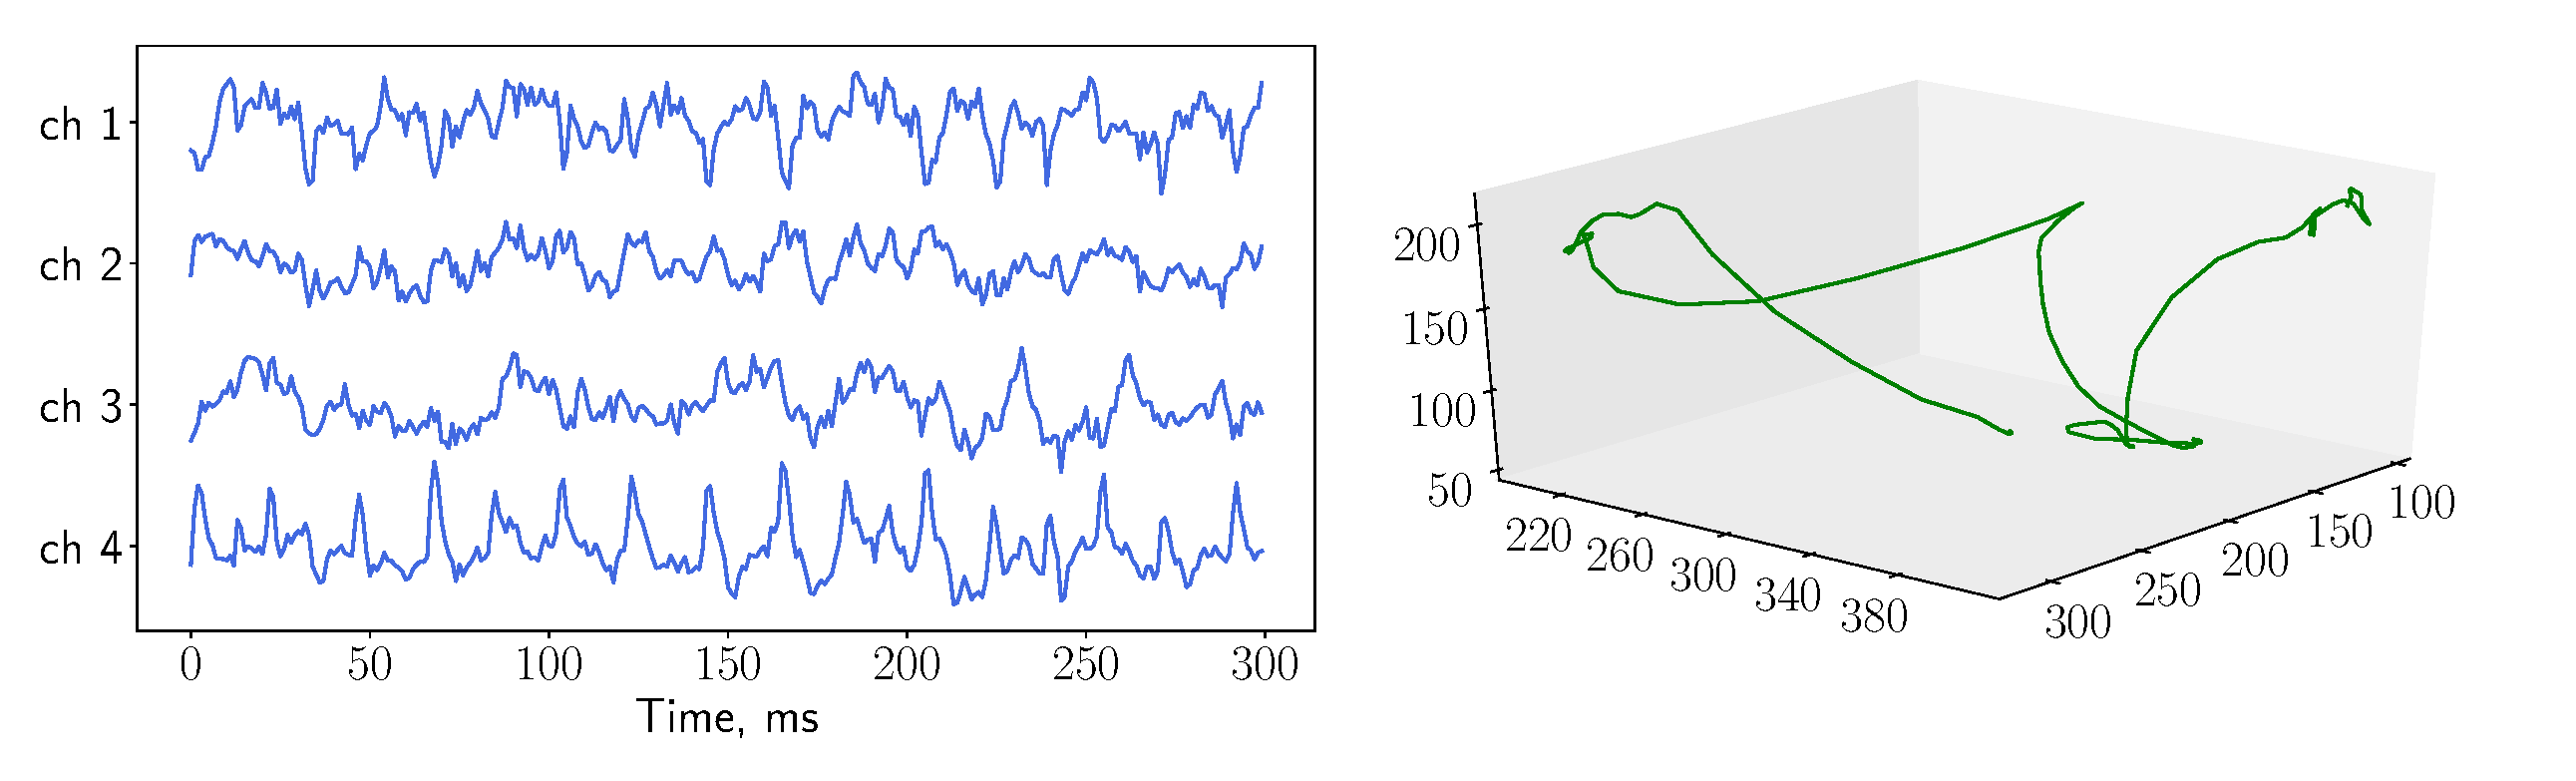
\includegraphics[width=\linewidth]{figs/ecog_data}
\end{figure}
\begin{minipage}{.55\linewidth}
\[
	\bX \in \bbR^{m \times (32 \cdot 27)}; \quad
	\bY \in \bbR^{m \times 3k}.
\]
\vspace{0.1cm}
\[
	\bY = 
	\begin{pmatrix}
	x_1 \,\, y_1 \,\, z_1 & \dots & x_{k\hphantom{+1}} \,\, y_{k\hphantom{+1}} \,\, z_{k\hphantom{+1}}\\
	x_2 \,\, y_2 \,\, z_2 & \dots & x_{k + 1} \,\, y_{k + 1} \,\, z_{k + 1}\\
	 \dots & \dots & \dots  \\
	x_m \, y_m \, z_m & \dots & x_{m + k} \, y_{m + k} \, z_{m + k}
	\end{pmatrix}
\]
\end{minipage}%
\begin{minipage}{.43\linewidth}
	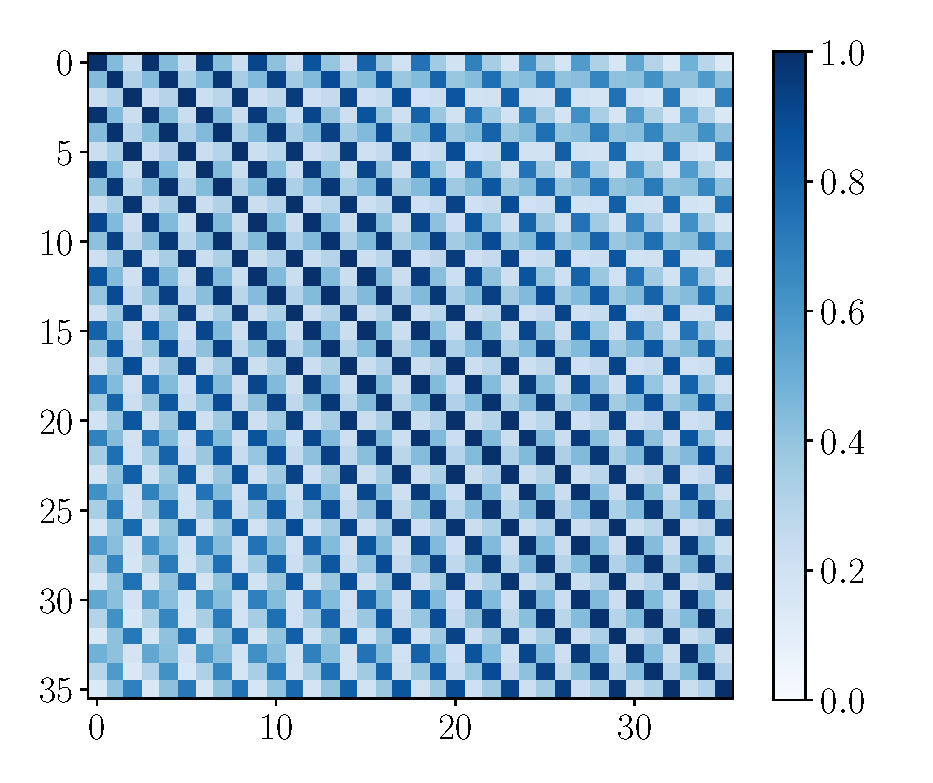
\includegraphics[width=\linewidth]{figs/Y_corr_matrix.eps}
	\begin{center}
		\vspace{-0.4cm}
		$\bY$ correlation matrix
		\vspace{-0.4cm}
	\end{center}
\end{minipage}
\vspace{0.5cm}

\hrulefill \\
\url{http://neurotycho.org}
\end{frame}
%--------------------------------------------------------------------------------
\begin{frame}{Quality criteria evaluation}
	\begin{figure}
		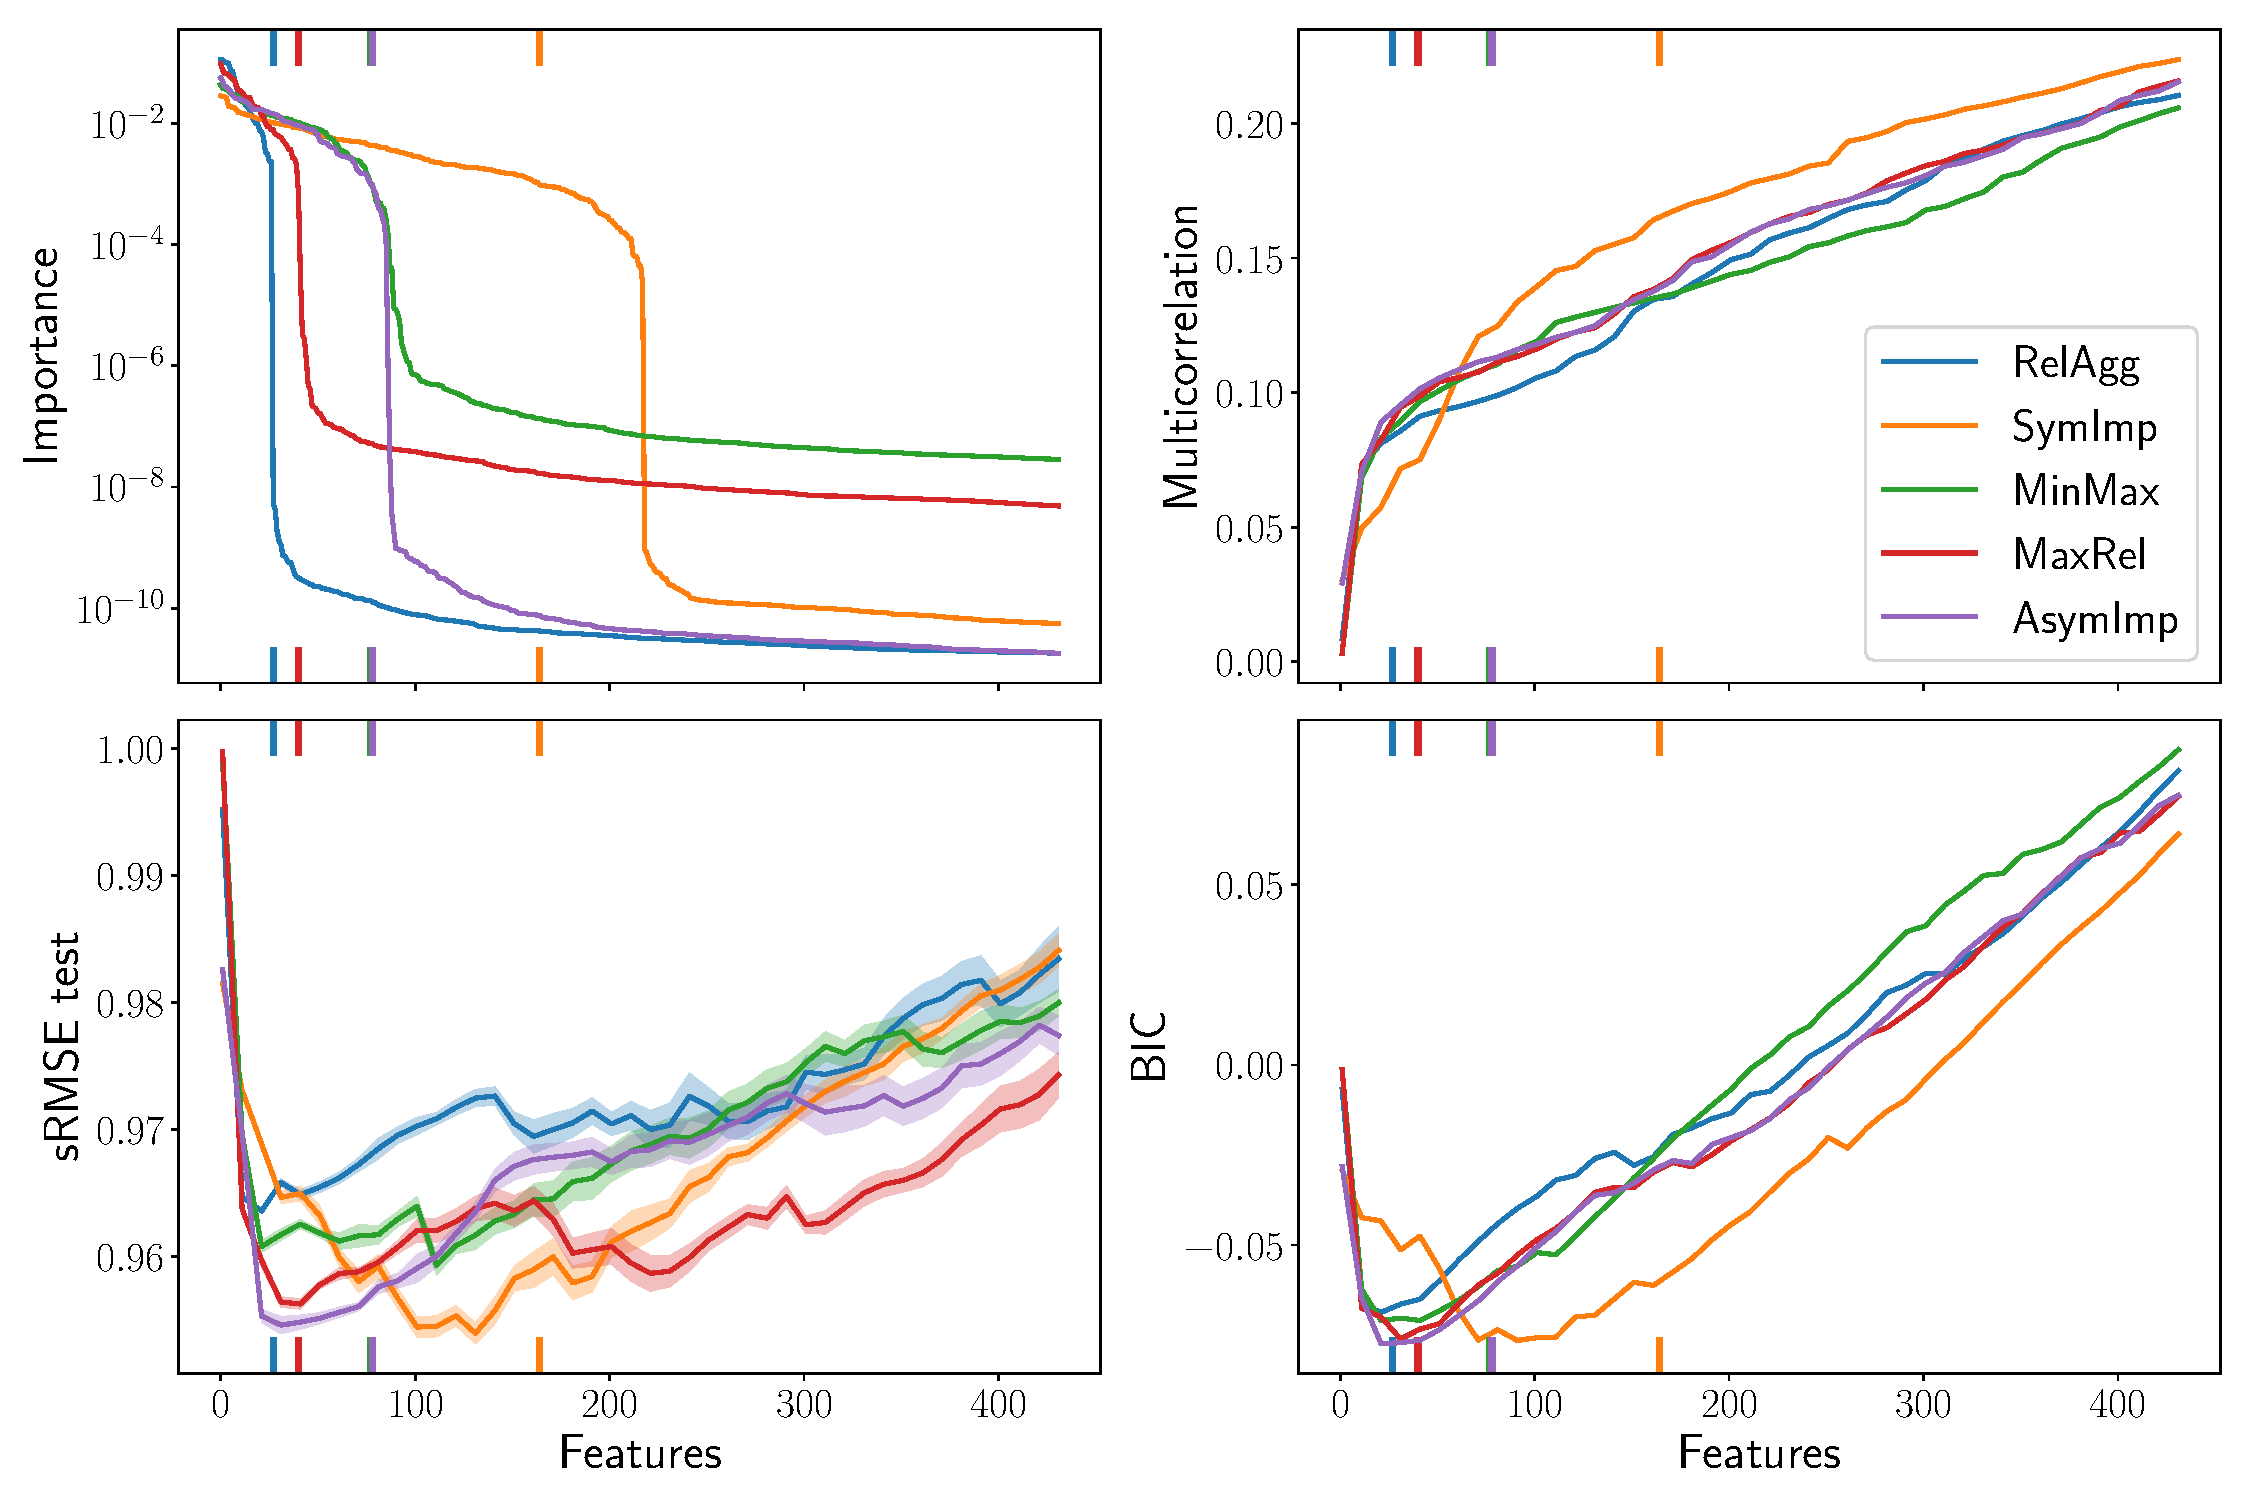
\includegraphics[width=\linewidth]{figs/ecog_3_30_metrics.pdf}
	\end{figure}
\end{frame}

%--------------------------------------------------------------------------------
\begin{frame}{Stability of selected feature subsets}
\begin{block}{Experiment design}
	\begin{itemize}
	\item generate bootstrap data
	\vspace{-0.1cm}
	\[
		(\bX, \bY) \rightarrow \bigl\{(\bX_1, \bY_1), \dots, (\bX_s, \bY_s)\bigr\};
	\]
	\item solve feature selection problem 
	\vspace{-0.1cm}
	\[
		 \bigl\{(\bX_1, \bY_1), \dots, (\bX_s, \bY_s)\bigr\}  \rightarrow \{\bz_1, \dots, \bz_s\};
	\]
	\item calculate statistics
	\vspace{-0.1cm}
	\end{itemize}
	\[
		\{\bz_1, \dots, \bz_s\} \rightarrow \{ \text{RMSE}, \|\ba\|_0, \text{Spearman }\rho, \ell_2 \text{ dist}\}.
	\]
\end{block}
\renewcommand{\arraystretch}{1.2}
\begin{table}[]
	\centering
	\begin{tabular}{l|ccccc}
		\hline
		& sRMSE  & $\|\ba\|_0$ & Spearman $\rho$ & $\ell_2$ dist \\ \hline
		RelAgg & 0.965 $\pm$ 0.002 & 26.8 $\pm$ 3.8 & 0.915 $\pm$ 0.016 & 0.145 $\pm$ 0.018   \\
		SymImp & 0.961 $\pm$ 0.001 & 224.4 $\pm$ 9.0 & 0.910 $\pm$ 0.017 & 0.025 $\pm$ 0.002   \\
		MinMax & 0.961 $\pm$ 0.002 & 101.0 $\pm$ 2.1& 0.932 $\pm$ 0.009 & 0.059 $\pm$ 0.004   \\
		MaxRel & 0.958 $\pm$ 0.003 & 41.2 $\pm$ 5.2 & 0.862 $\pm$ 0.027 & 0.178 $\pm$ 0.010   \\
		AsymImp & 0.955 $\pm$ 0.001 & 85.8 $\pm$ 10.2& 0.926 $\pm$ 0.011 & 0.078 $\pm$ 0.007  \\ \hline
	\end{tabular}
\end{table}
\end{frame}
%--------------------------------------------------------------------------------
\begin{frame}{QPFS vs PLS}

\begin{block}{Design of experiment}
	To compare feature selection and dimensionality reduction for linear regression and PLS regression models.
\end{block}

\begin{figure}[h]
	\begin{minipage}{.5\linewidth}
		\centering
		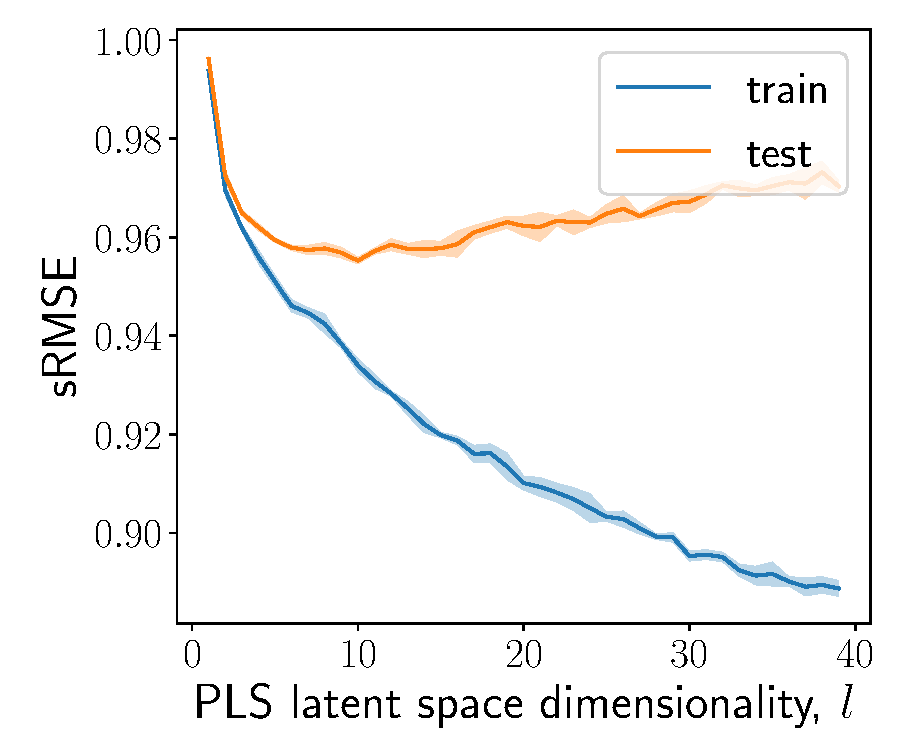
\includegraphics[width=1.\linewidth]{figs/pls_vs_k}
	\end{minipage}%
	\begin{minipage}{.5\linewidth}
		\centering
		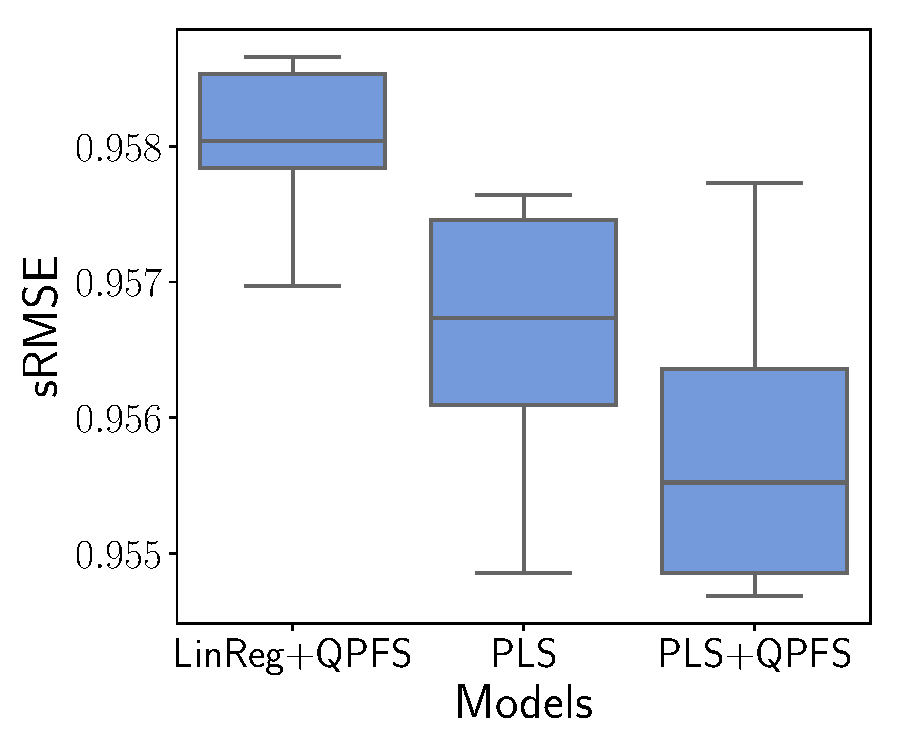
\includegraphics[width=1.\linewidth]{figs/models}
	\end{minipage}
\end{figure}

\end{frame}
\begin{frame}{Results}
\begin{itemize}
	\item The problem of ECoG signal decoding in high dimensional spaces is investigated.
	\vfill
	\item Dimensionality reduction technique with space structure analysis is investigated.
	\vfill
	\item Feature selection methods which take into accout structure of both input and target spaces are proposed.
	\vfill
	\item The combination of feature selection and dimensionality reduction is proposed.
	\vfill
	\item Proposed feature selection algorithms give the stable and adequate solutions.
\end{itemize}
\end{frame}
%--------------------------------------------------------------------------------
\begin{frame}{Conclusion}
\begin{block}{Publications}
\vspace{-0.1cm}
\begin{itemize}
	\item Isachenko R., Strijov V. Metric learning for time series multiclass classification \emph{Informatics and Applications}, 10(2), 2016.
	\item Isachenko~R. et al. Feature Generation for Physical Activity Classification. \emph{Artificial Intellegence and Decision Making}, 2018, submitted to the journal.
	\item Isachenko~R., Strijov~V. Quadratic programming optimization for Newton method. \emph{Lobachevskii Journal of Mathematics}, 2018, accepted to the journal.
	\item Isachenko~R., Strijov~V. Dimensionality reduction for multivariate ECoG-based data. \emph{Chemometrics}, 2018, ready for submission.
\end{itemize}
\end{block}
\vspace{-0.1cm}
\begin{block}{Conferences}
\vspace{-0.2cm}
\begin{itemize}
	\item Lomonosov, 2016, Moscow. Metric learning in multiclass time series classification.
	\item Intelligent Data Processing Conference, 2016, Barcelona. Multimodel forecasting multiscale time series in internet of things.
	\item MMRO, 2017, Taganrog. Local models for classification of complex structured objects.
\end{itemize}
\end{block}
\end{frame}
\end{document} 
